% \section{Preliminary}
% \label{sec:preliminary}

% \textbf{Ladder Side Tuning}\cite{sung2022lst} trains a ladder side network, a small and separate network that takes intermediate activations from the backbone transformer as input and makes predictions. It includes a downward projection $h_i^f=x_iW_d^T$ to decrease dimension of the feature and a gated connection to integrate the intermediate activation of the backbone $f$ and the features of the side network $g$ Adaptively. The output is calculated by
% \begin{equation}
%     \boldsymbol{h}_{i}^{g}=\Phi(\mu_{i} * \boldsymbol{h}_{i}^{f}+\left(1-\mu_{i}\right) * \boldsymbol{h}_{i-1}^{g})
% \end{equation}
% where $\mu_{i}=\operatorname{sigmoid}\left(\frac{\alpha_{i}}{T}\right)$ is a gate parameterized with a learnable zero-initialized scalar $\alpha_i$ and temperature $T$(= 0.1), $\Phi$ is a linear layer that projects the fused features.

% \textbf{Prompt tuning}\cite{li2021prefix,jia2022visual} freezes the backbone network during fine-tuning while inserting learnable tokens into the input token sequence. Prompt tokens interact with the original tokens through attention mechanisms. Given the class token $x_{cls}\in R^{1 
% \times d}$ and patch tokens $T \in R^{N \times d}$, where $N$ is the num of patch tokens, we can insert prompt tokens $P_i \in R^{n \times d}$ for each layer following VPT-Deep\cite{jia2022visual}, where $n \ll N$ is the num of prompt tokes.The output of $i$-th layer($L(\cdot)$) is expressed as follows:
% \begin{equation}
%     \boldsymbol{x}_{i}=L_{i}\left(\left[\boldsymbol{T}_{c l s} ; \boldsymbol{P}_{i} ; \boldsymbol{T}\right]\right)
% \end{equation}

\begin{figure*}
    \centering
    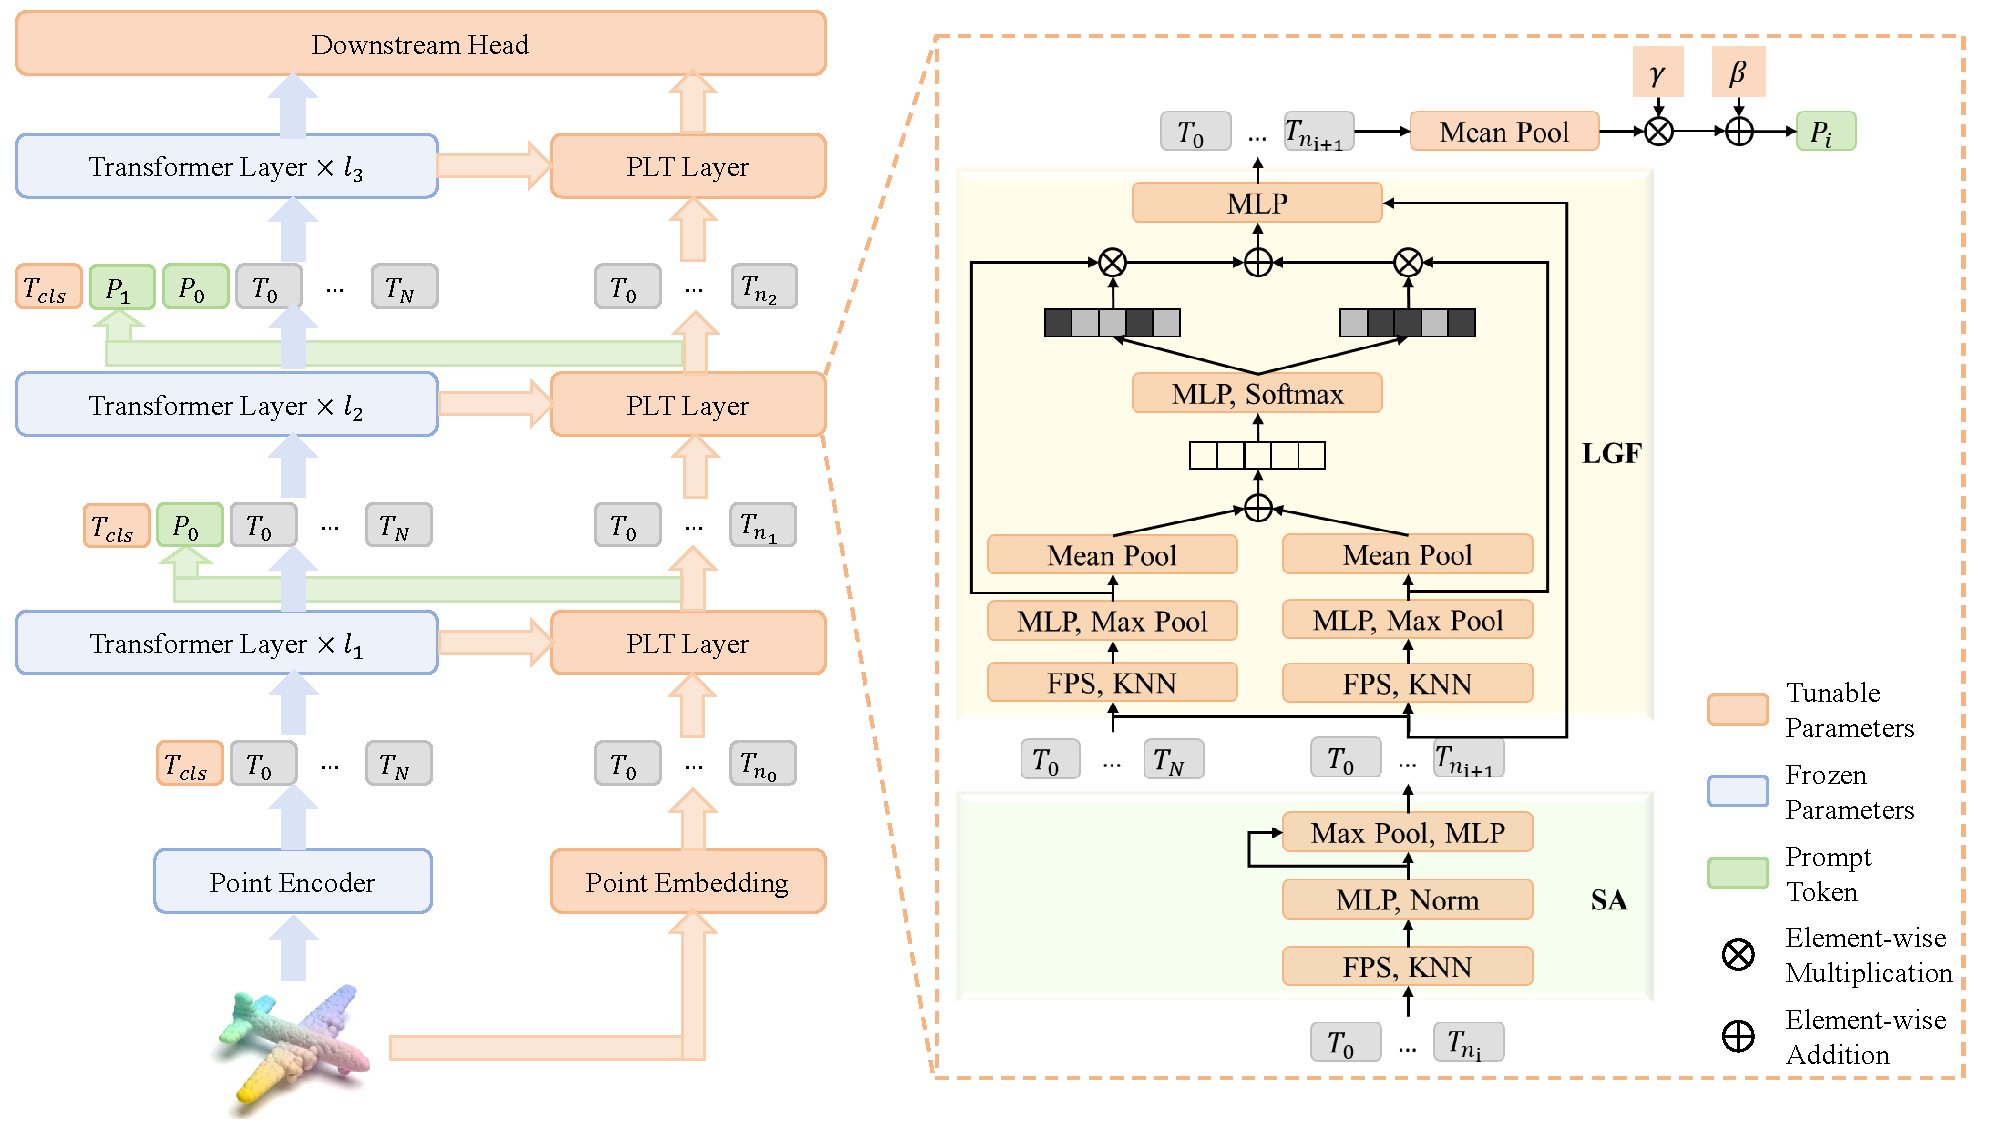
\includegraphics[width=\linewidth]{fig/Overall.pdf}
    \caption{The overall of our PLT. During fine-tuning, we froze the pre-trained backbone network and only fine-tune the PLT branch and the class token. The PLT branch consists of two main components: 1) Set Abstraction (SA), and 2) Local-Global Fusion Module (LGF).
}
    \label{fig:overall}
\end{figure*}

\section{Methodology}
\label{sec:methodology}
%Fine-tuning a pre-trained model has achieved impressive results, but it requires a significant training cost.To address this, We combine ladder side tuning with prompt tuning to propose a novel point cloud fine-tuning method called Point Ladder Tuning (PLT), which achieves a better balance between performance and parameter efficiency for 3d point cloud learning. The overall framework is illustrated in Fig..In our method, we introduce a hierarchical ladder network based on LST to extract local information from the raw input and fuse it with the global intermediate activations of the backbone network through a local-global fusion module(LGF). To further enhance performance, we also generate prompt tokens derived from the fused features, which are used to fine-tune the global features of the backbone network.



%Fine-tuning pre-trained models has demonstrated remarkable success across various domains, yet it often comes with high computational and storage costs. To address this issue, we propose Point Ladder Tuning (PLT), a novel fine-tuning approach that combines the strengths of Ladder Side Tuning (LST) and prompt tuning to achieve a more efficient balance between performance and parameter usage for 3D point cloud learning. 


%LST primarily focuses on statically weighting and fusing the global intermediate activations from each layer, neglecting the equally critical local information essential for downstream tasks. This limitation leads to suboptimal performance, particularly in point cloud neighborhoods where local features play a crucial role. On the other hand, Prompt Tuning suffers from the issue of randomly initializing the Prompt Token, which makes optimization significantly more challenging. Additionally, once trained, the Prompt Token remains fixed across all instances, lacking the adaptability needed to capture instance-specific variations. This lack of adaptability further contributes to degraded performance, as the model fails to effectively adjust to the diverse characteristics present in different data instances.

%In contrast to these methods, our PLT addresses these limitations by incorporating both global and local features effectively, ensuring better optimization and adaptability to individual instances, which ultimately leads to improved performance in complex tasks like point cloud semantic segmentation.

%At the core of PLT, we introduce a hierarchical Ladder Network based on LST, which extracts local features directly from the raw input point cloud. These local features are then integrated with the global intermediate activations of the pre-trained backbone network through a Local-Global Fusion (LGF) module, facilitating the creation of multi-scale representations. To further improve performance, we generate prompt tokens from the fused local-global features, which are then used to fine-tune the global features of the backbone network. This approach significantly reduces the number of parameters that need to be updated, while retaining the rich semantic knowledge acquired during pre-training, thereby enhancing task-specific performance across various point cloud applications. Through this method, we offer a more computationally efficient solution without compromising the effectiveness of the pre-trained model.


Fine-tuning pre-trained models, though effective across domains, often incurs high computational and storage costs. To address this, we propose Point Ladder Tuning (PLT), an efficient fine-tuning approach for 3D point cloud learning that combines Ladder Side Tuning (LST) and prompt tuning to optimize parameter efficiency and task performance. While LST statically weights global activations but overlooks crucial local features, and prompt tuning lacks adaptability across instances, PLT integrates both local and global features to enhance optimization and adaptability.

PLT introduces a hierarchical Ladder Network to extract local features directly from the input point cloud, which are fused with the backbone’s global activations via a Local-Global Fusion (LGF) module, creating multi-scale representations. Further, dynamic prompt tokens generated from these fused features refine the backbone’s global features, achieving high task-specific performance with minimal parameter updates. This approach thus maintains the semantic richness of pre-trained models while substantially reducing computational demands, demonstrating effectiveness across point cloud applications like semantic segmentation.
Our framework is shown in Fig.~\ref{fig:overall2}.

\subsection{Hierarchical Ladder Network}
Pre-trained models typically learn the global information of input point clouds through attention mechanisms but often overlook the importance of locality, which is crucial for downstream tasks, especially dense prediction tasks. Although Point PEF introduces a Geometry-Aware Adapter to capture local information, it still relies on the global intermediate activations of pre-trained models, which limits its ability to effectively learn local features within the original point cloud. Additionally, because pre-trained models often operate at a single scale throughout the learning process, lacking multi-scale information, this constraint further impedes performance on downstream tasks.

To address these problems, we introduce a hierarchical Ladder network to better capture the intrinsic local information of the input point cloud. The module includes multiple PLT layers that are capable of capturing point cloud features at different scales, which has been shown to be effective in subsequent experiments. The PLT Layer consists of two main components: 1) Set Abstraction (SA), and 2) Local-Global Fusion Module (LGF).

Given the input point cloud $P \in R^{N \times 3}$, where N is the num of the input point cloud, we first apply Point Embedding to map it into a high-dimensional space, obtaining the point cloud feature $F \in R^{N \times C}$, where is the dimension of the point cloud feature. Next, we use Set Abstraction (SA) to perform downsampling. This process begins with farthest point sampling (FPS) to select a set of center points $C=\{c_1, \ldots, c_n\}$. Then, we use k-nearest neighbors (KNN) to construct local neighborhoods $P(c)=\{p^1_c, \ldots,  p^k_c\}$, $F(c)=\{f^1_c, \ldots, f^k_c\}$ for each center point $c$. Finally, we apply max pooling followed by a multi-layer perceptron (MLP) to obtain the output point cloud. The formula for this process is as follows:
\begin{flalign}
    \boldsymbol{f}_{c} & = \varphi \left(\left[\boldsymbol{f}_{c}^{j} ;\left(\boldsymbol{p}_{c}-\boldsymbol{p}_{c}^{j}\right)\right]\right)\\
    \boldsymbol{f}_{c}^{'} & = \boldsymbol{f}_{c} + \rho \left( h_{\boldsymbol{\Theta}}\left ( \boldsymbol{f}_{c} \right) \right)
\end{flalign}
where $\rho$ and $\varphi$ represent a MLP respectively, $[\cdot, \cdot]$ represents concat operation. And $h_{\boldsymbol{\Theta}}$ represents the aggregation function. Unless otherwise specified, we use Max-Pooling.

\subsection{Local-Global Fusion Module}
To make better use of the local information captured in the PLT Branch and the global information captured in the pre-trained backbone network, we propose a local-global fusion module that adaptively aggregates both types of information through selective attention. Given the input point cloud $P_{s}$ and their corresponding features $F_{s}$ from the PLT layer, as well as the output point cloud $P_{m}$ and its corresponding features $F_{m}$ from the backbone network, we firstly use $W$ to map the output features of the backbone network to match the same feature dimension as the input point cloud feature vectors of the PLT layer:
\begin{equation}
    \boldsymbol{F}_{m}^{'} = \boldsymbol{F}_mW 
\end{equation}

Next, we use the same operations as Set Abstraction (SA) to extract both the global features $F_g$, which are derived from the interaction between the input point cloud $P_s$ of the PLT layer and the output point cloud $P_m$ of the backbone network, and the local features $F_l$, which are obtained from the interaction between the input point clouds $P_s$ of the PLT layer.

Finally, we apply a selective attention mechanism to adaptively fuse the global and local features. This mechanism allows the model to focus on the most relevant information from each source, ensuring that both global context and fine-grained local details are effectively integrated. Firstly, we apply the aggregation function $\mathcal{A}$, with average pooling as the default, to the global and local features to obtain the corresponding global and local feature vectors:
\begin{equation}
    \boldsymbol{f}_g, \boldsymbol{f}_l = \mathcal{A}(\boldsymbol{F}_g),  \mathcal{A}(\boldsymbol{F}_l)
\end{equation}

Then, we add the global and local features and pass them through a MLP to obtain $z_g$ and $z_l$:
\begin{equation}
    \boldsymbol{z}_g, \boldsymbol{z}_l = \alpha \left( \boldsymbol{f}_g + \boldsymbol{f}_l \right)
\end{equation}
where $\alpha$ represents a MLP.

Next, we apply Softmax to compute the attention weights $s_g$ and $s_l$ for the global and local features:
\begin{equation}
    \boldsymbol{s}_g^i = \frac{e^{\boldsymbol{z}_g^i}}{e^{\boldsymbol{z}_g^i} + e^{\boldsymbol{z}_l^i}}, \boldsymbol{s}_l^i = \frac{e^{\boldsymbol{z}_l^i}}{e^{\boldsymbol{z}_g^i} + e^{\boldsymbol{z}_l^i}}
\end{equation}

Subsequently, the global and local features are weighted according to their attention scores to produce the fused multi-scale features:
\begin{equation}
    \boldsymbol{F}_{ms} = \boldsymbol{s}_g \boldsymbol{F}_g + \boldsymbol{s}_l \boldsymbol{F}_l
\end{equation}

Finally, we use an MLP $\tau$ to perform feature mapping and add the result to the input features:
\begin{equation}
     \boldsymbol{F}_{o} = \boldsymbol{F}_s + \tau \left( \boldsymbol{F}_{ms} \right)
\end{equation}

By selectively emphasizing the most relevant local and global features through attention, our LGF ensures the effective integration of both types of information, enhancing the model's ability to capture multi-scale features. This is crucial for tasks that require a balance between fine-grained local details and the broader global structure of point clouds, especially in dense prediction tasks.

\subsection{Fine-tuning on the Backbone Network}
To enable the pre-trained backbone network to generate more effective global features for downstream tasks, we propose a dynamic prompt generation method based on the multi-scale point cloud features output $F_{o}$ by the Local-Global Fusion (LGF) module. Firstly, $F_{o}$ is mean-pooled to obtain a compact representation. These pooled features are then scaled and translated using learnable parameters $\gamma$ and $\beta$ to generate multi-scale prompt $p$. To efficiently utilize parameters, we reuse $W$ to align the dimensions of the multi-scale prompts with the dimensions of the backbone network features. The formula can be expressed as follows:
\begin{equation}
    p = \left( \boldsymbol{\gamma} \times \frac{1}{n}\sum_i^n{\boldsymbol{F}_{o}^i} + \boldsymbol{\beta} \right) W^T
\end{equation}
where n is the num of tokens in $F_o$.

Finally, we incorporate multi-scale prompts into the backbone network for learning. The output of the $l$-th transformer layer $x_l$ can be expressed as
\begin{equation}
    \boldsymbol{x}_l=L_l\left(\left[\boldsymbol{T}_{c l s} ; \boldsymbol{p}_{0}, \ldots, \boldsymbol{p}_{i-1} ; \boldsymbol{T}\right]\right)
\end{equation}

To enhance performance further, we follows ssf\cite{lian2022scaling} and applies scaling and shifting to the output of each module within the backbone network, enabling the extraction of task-specific global information. Given an input $x$, the output $y$ can be expressed as:
\begin{equation}
    \boldsymbol{y} = \boldsymbol{s} \times \boldsymbol{x} + \boldsymbol{t}
\end{equation}
where s and t represents scaling and shifting parameter respectively, which are learnable.
